\begin{tcolorbox}[
    colback=green!5!white, % Very light red background (5% red, 95% white)
    colframe=darkgreen!40!white, % Light red border (30% red, 70% white)
   title=Motivation, % Optional title
    fonttitle=\bfseries % Bold title
    ]
    Neoclassical growth models treat technological progress as exogenous, leaving the main driver of long-run growth unexplained. Endogenous growth theory addresses this by modeling innovation, human capital accumulation, and knowledge spillovers (“externalities”) as outcomes of economic decisions. This allows productivity growth to arise within the model, driven by investment, learning, and creative destruction.\\\\
    Endogenous growth models build a consistent framework for economic growth driven by \textbf{investment in physical capital}, human capital, and \textbf{R\&D}, without relying on an exogenous process. 
  
\end{tcolorbox}

\subsection{The simplest form of endogenous growth: AK Model}
\noindent The \textbf{AK-Model} refers to a production function of the form $Y=AK$ which is obtained if one starts from Cobb-Douglas and $\alpha$ approaches $1$:
$$Y=AK^\alpha L^{1-\alpha} \xrightarrow{\alpha \rightarrow 1}Y=AK$$
\par\noindent{\color{lightgray}\rule{\linewidth}{0.4pt}}
In the \textbf{Ramsey Model} the Keynes Ramsey Rule (KRR) with an AK production function becomes $\hat{C}^*=  \hat{Y}^*=\frac{A-\delta-\rho}{\sigma}$. Consumption and tuhs output grow, if $A-\delta-\rho>0$. We will see that due to the AK production function, policy can influence $A$ in this  and thereby influence growth: \\\\
Since $r+\delta=\frac{\partial Y}{\partial K}$ \textit{(this is a general result, see chapter 1)} we get $\frac{\partial Y}{\partial K}=r+\delta$, due to $Y=AK$, we see that $\frac{\partial Y}{\partial K}=A=r+\delta$. Thus, policymakers can, by influencing $r$, influence $A$ which makes $A$ endogenous. 
\par\noindent{\color{lightgray}\rule{\linewidth}{0.4pt}}
In the \textbf{Solow Model} the steady state is characterized by $\dot{K}=sY-\delta K$ which yields the steady state growth rate (balanced growth path): $\hat{K}^*=sY/K-\delta=\hat{Y}^*$. Plugging in the AK production function here, yields: $\hat{K}^*=sA-\delta=\hat{Y}^*$ and growth is positive, if $sA-\delta>0$. Following the same argument as above, the policymaker can influence $A$ through $r$ and thereby the model features endogenous growth.
\subsection{Romer (1986): Simple Endogenous Growth Model}

\textbf{Households.} A representative (mass one) Ramsey household with inelastic labor supply $L$ and assets $\mathcal{A}(t)$ earns income
\[
w(t)L + r(t)\mathcal{A}(t).
\]
Consumption evolves according to the Keynes--Ramsey rule
\[
\frac{\dot{c}(t)}{c(t)} = \frac{r(t) - \rho}{\sigma}.
\]

\noindent \textbf{Firms.} A continuum of firms $i \in [0,1]$ produces output with technology
\[
Y(i,t) = K(i,t)^{\alpha} \bigl[A(t)L(i)\bigr]^{1-\alpha}, \quad \alpha \in (0,1), \ \delta \in (0,1).
\]
Aggregate technology features Marshallian externalities ('spill-overs across firms'):
\[
A(t) = \int_0^1 K(i,t)\, di. 
\]

\noindent \textbf{Each firm solves:} $\max_{K(i),L(i)} \; K(i)^{\alpha}[A L(i)]^{1-\alpha} - wL(i) - (r+\delta)K(i)$ and we obtain the following FOCs:
\[
(1-\alpha)K(i)^{\alpha}[A L(i)]^{-\alpha}A - w = 0,
\]
\[
\alpha K(i)^{\alpha-1}[A L(i)]^{1-\alpha} - (r+\delta) = 0.
\]

\noindent \textbf{In symmetric equilibrium we have:} $K(i)=K$, $L(i)=L$ $\forall$ $i$ and hence $A = \int_0^1 K(i)\,di = K.$\\\\
Rewriting the FOC for capital:
\[
\alpha K^{\alpha-1}(K L)^{1-\alpha} = r+\delta \;\;\Rightarrow\;\; r(t) = \alpha L^{1-\alpha} - \delta.
\]
And combining with the \textbf{market clearing} conditions: 
\[
\int_0^1 L(i)\,di = L, \qquad \int_0^1 K(i,t)\,di = \mathcal{A}(t),
\]
$($which imply the aggregate resource constraint $\dot{K}(t) = Y(t) - \delta K(t) - C(t))$ yield the \textbf{balanced growth path} after plugging $r(t) = \alpha L^{1-\alpha} - \delta$ into the KRR from above: 
\[
\left(\frac{\dot{c}}{c}\right)^* = \left(\frac{\dot{K}}{K}\right)^* = \left(\frac{\dot{Y}}{Y}\right)^* = \frac{\alpha L^{1-\alpha} - \delta - \rho}{\sigma}.
\]
\noindent \textbf{The key implication} is that knowledge spillovers ($A(t)=K(t)$) eliminate diminishing returns to capital at the aggregate level, generating endogenous growth with a constant equilibrium interest rate. Without these knowledge spillovers the typical chain of effects is: $K\uparrow \rightarrow r\downarrow \rightarrow s\downarrow$, but here an increase in $K$ also increases $A$, thus: $K\uparrow \rightarrow A\uparrow \rightarrow r\uparrow \rightarrow s \uparrow$. This second chain of effects offsets the decrease in $s$ and may lead to forever ongoing capital accumulation. In other words: The marginal product of capital is not diminished, i.e. it does not fall \textit{(as strongly?, im unsure here)} as $K$ increases. This is somewhat similar to the AK-model effect.
\par\noindent{\color{lightgray}\rule{\linewidth}{0.4pt}}

\subsubsection{A Note on Marshallian Externalities}


\textbf{Concept:} Marshallian externalities imply that a firm's efficiency increases with the intensity of surrounding economic activity. While internal production remains standard, Total Factor Productivity (TFP) is endogenized as a function of the aggregate environment.
\\\\
\noindent \textbf{Firm-Level Production:}
Individual firm $i$ produces according to:
\begin{equation}
    Y(i) = B K(i)^\alpha L(i)^{1-\alpha}
\end{equation}

\noindent \textbf{Endogenous TFP (The Modeling Shortcut):}
TFP ($B$) is assumed to depend on the average capital ($\bar{K}$) and average labor ($\bar{L}$) across all firms:
\begin{equation}
    B = A \bar{K}^\beta \bar{L}^\gamma \quad (\beta, \gamma \geq 0)
\end{equation}

\noindent Substituting this into the production function yields:
\begin{equation}
    Y(i) = A \bar{K}^\beta \bar{L}^\gamma K(i)^\alpha L(i)^{1-\alpha}
\end{equation}

\noindent \textbf{Key Insights:}
\begin{itemize}
    \item \textbf{Returns to Scale:} Production exhibits \textbf{CRS} in private inputs ($K(i), L(i)$), allowing for perfect competition, but \textbf{IRS} in aggregate inputs due to the externalities.
    \item \textbf{Special Case:} The previous model (Romer 1986) is a restricted version of this framework where $A=1$, $\gamma=0$, and $\beta=1$ (yielding $B = \bar{K}$).
\end{itemize}

\subsection{Romer (1990): R\&D driven growth}
The model rests on three premises: 
\begin{itemize}
    \item Economic growth is driven by \textbf{technological progress} as well as \textbf{capital accumulation}.
    \item Technological progress results from deliberate actions
taken by private agents who respond to \textbf{market
incentives}. 
    \item Technological knowledge is a \textbf{non-rivalrous input}.
\end{itemize}


\subsubsection{Modelling Technological Change}
Final output is produced according to $Y = F(A, K, L)$, which exhibits constant returns to scale (CRS) in private inputs $K$ and $L$, i.e. $ F(A, \lambda K, \lambda L) = \lambda Y$ for any $ \lambda \geq 0.$ Furthermore $\frac{\partial F}{\partial X} > 0$ and
$\frac{\partial^2 F}{\partial X^2} < 0$ for all $X \in \{A, K, L\}$. Under perfect competition, each factor is rewarded with its marginal product
$F_X(\cdot) := \frac{\partial F}{\partial X}$, so by Euler's theorem output is
fully exhausted:
\begin{equation}
    Y = \underbrace{F_K(\cdot)}_{r+\delta} K + \underbrace{F_L(\cdot)}_{w} L.
\end{equation}

\noindent This reveals a fundamental tension: \textbf{perfect competition, CRS, and
premise (2) are mutually exclusive}. Agents who produce technological change must
respond to market incentives and therefore need to be rewarded. Yet under CRS and
perfect competition, \textbf{output is entirely used up paying wages and rental rates,
leaving nothing to compensate researchers}.
\\
\subsubsection{Structure of the model}

\begin{minipage}[t]{0.48\textwidth}
    \textbf{Households}
    \begin{itemize}
        \item Supply labour inelastically
        \item Split income into consumption and saving
        \item Lend capital to $x$ firms (physical capital and purchase of blueprints)
    \end{itemize}
\end{minipage}
\hfill
\begin{minipage}[t]{0.48\textwidth}
    \textbf{Production side: 3 sectors}
    \begin{itemize}
        \item Final-output sector $Y$ (perfect competition)
        \item Intermediate goods sector $x(i)$(monopolistic competition)
        \item R\&D sector (perfect competition)
    \end{itemize}
\end{minipage}
\begin{figure}[H]
    \centering
    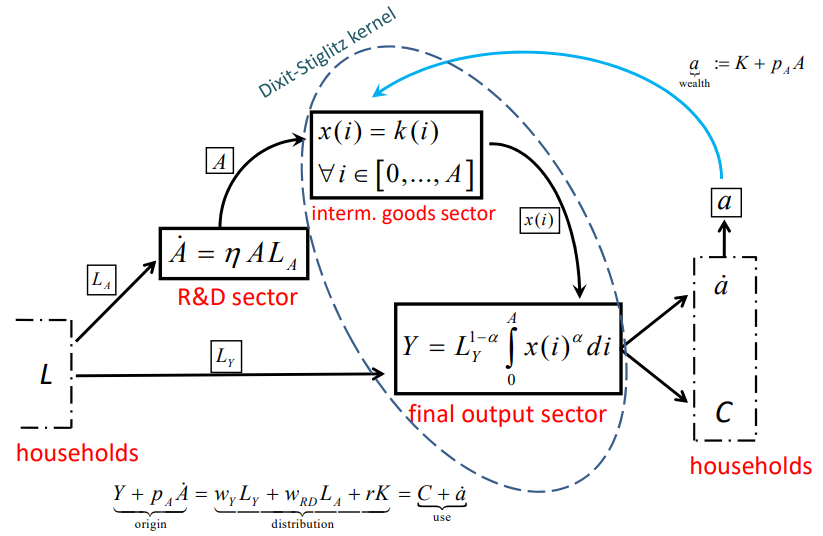
\includegraphics[width=0.6\linewidth]{image.png}
\end{figure}


\noindent The Dixit-Stiglitz kernel refers to the goods sector featuring many intermediate goods $x(i)$ which are \textbf{imperfect substitutes} and a final output sector which bundles the intermediate goods into the final output $Y$. The production function of the \textbf{monopolistic} intermediate firms are $x(i)=k(i)$, i.e. one unit of capital is used to produce one unit of intermediate good. 



\subsubsection{Households: \textit{Ramsey household with two assets.}}
The economy is populated by a \textbf{continuum of mass one} of identical households. Each household is endowed with $L$ units of labor services per unit of time, which are supplied \textbf{inelastically} to the labor market.
\begin{itemize}
    \item Household wealth comprises \textbf{equity} ($p_A A$) and \textbf{raw capital} ($K$):
    \[
        a = p_A* A + K.
    \]
    \begin{itemize}
        \item $A$ is the number of intermediate good firms and $p_A$ is the respective price, thus $p_A* A$ is equity (Aktienvermögen)
        \item Revenues from issuing shares are used by the $x$-firm to purchase a blueprint.
        \item In equilibrium, the price of a blueprint equals the value of the firm.
        \item Raw capital $K$ is rented out to the $x$-firms.
    \end{itemize}
    \item The household chooses the consumption path $C(t)$ to maximize discounted utility:
    \[
        \max \int_0^\infty \frac{C(t)^{1-\sigma}-1}{1-\sigma}\, e^{-\rho t}\, dt.
    \]
    \item Optimal consumption obeys the \textbf{Keynes-Ramsey rule} (KRR):
    \[
        \frac{\dot{C}(t)}{C(t)} = \frac{r-\rho}{\sigma}.
    \]
\end{itemize}


\begin{tcolorbox}[
    colback=blue!1!white, % Very light red background (5% red, 95% white)
    colframe=blue!40!white, % Light red border (30% red, 70% white)
   title=The value of a firm, % Optional title
    fonttitle=\bfseries % Bold title
    ]

This gives firms a positive value: $p_A$ represents the value of the infinite discounted income stream of the firm. Note that in standard neoclassical theory, firms do not make profits in equilibrium, so the value of the firm would be zero, which is not the case here.

\end{tcolorbox}


\subsubsection{Final-output sector}

The final-output sector ($Y$-sector) consists of firms producing a homogeneous good $Y$ under \textbf{perfect competition}. The production technology is given by
\[
    Y = L_Y^{1-\alpha} \int_0^A x(i)^\alpha \, di 
\]
where $i \in [0,A]$ is the index of intermediate goods, $A$ denotes the ``number'' of types of intermediate goods, and $x(i)$ is the quantity of intermediate goods of type $i$.

\begin{itemize}
    \item Note that the intermediate goods are \textbf{machines}: they serve as input factors for the final-good firm (think of shovels, pickaxes, machines, etc.). Intermediate goods are \textbf{not} consumption goods, and the final firm is not a ``goods bundler''
    \item $A$ represents the number of intermediate firms, i.e. machines in the economy. A larger $A$ means more intermediate firms with different technologies, which raises $Y$.
\end{itemize}

\noindent \textbf{Reduced-form technology.} Imposing a symmetric equilibrium $x(i) = x \;\forall\, i \in [0,\dots,A]$ and the market-clearing condition for raw capital ($K = Ak = Ax$), the production function reduces to
\[
    Y = L_Y^{1-\alpha} \int_0^A x(i)^\alpha \, di 
    \;\xrightarrow{\;x(i)=x\;} \; 
    Y = L_Y^{1-\alpha} A x^\alpha 
    \;\xrightarrow{\;K=Ax\;} \; 
    Y = (A L_Y)^{1-\alpha} K^\alpha.
\]

\begin{itemize}
    \item This is a \textbf{Cobb-Douglas technology with labor-augmenting technical change}.
    \item Increasing $A$ while holding $K = Ax$ constant (by reducing $x$ as $A$ rises, i.e. there are more smaller firms) boosts the productivity of labor.
    \item The technology captures the basic idea that \textbf{``division of labor and specialization''} makes production more efficient
    \item The constraint $K = Ax$ is crucial: it shows that the result ``more $A$ is better'' holds \textbf{even though the total amount of input factor is fixed}. With $A = 1$, diminishing returns set in much faster than with, say, $A = 3$ specialization across more varieties delays the curvature of the production function.
\end{itemize}

\subsubsection{Intermediate goods sector}

The intermediate goods sector consists of producers who manufacture \textbf{differentiated intermediate goods} $x(i)$. The production technology is
\[
    x(i) = k(i),
\]
i.e., it takes one unit of ``raw capital'' to produce one unit of any $x(i)$. This is a trivial \textbf{constant-returns-to-scale} production function. \textbf{The marginal cost of any $x$ therefore equals $r$, the rental price of capital.}

\begin{itemize}
    \item Before producing and marketing $x$, firms must purchase a \textbf{blueprint} (design). The blueprint acts as a \textbf{fixed cost of market entry}: a firm needs a blueprint in order to produce a new machine. 
    \item The $x$-market is \textbf{monopolistically competitive}: there is a large number of producers (one producer per variety) offering imperfect substitutes.
    \item $x$-producers sell intermediate goods $x(i)$ to $Y$-producers by charging a price $p(i)$.
\end{itemize}

\noindent \textit{Note:} The $x(i)$ are symmetric with regard to production technology and with regard to the way they enter into the production function of the final-output good. They are differentiated only in the sense that they are considered \textbf{imperfect substitutes} from the user's perspective, implying that ``convex combinations are superior''.

\paragraph{Flow of payments between HH, $x$-producer, and $Y$-producer.}
The interaction between households, intermediate-goods producers, and final-output producers can be summarized as a circular flow:

\begin{figure}[H]
    \centering
    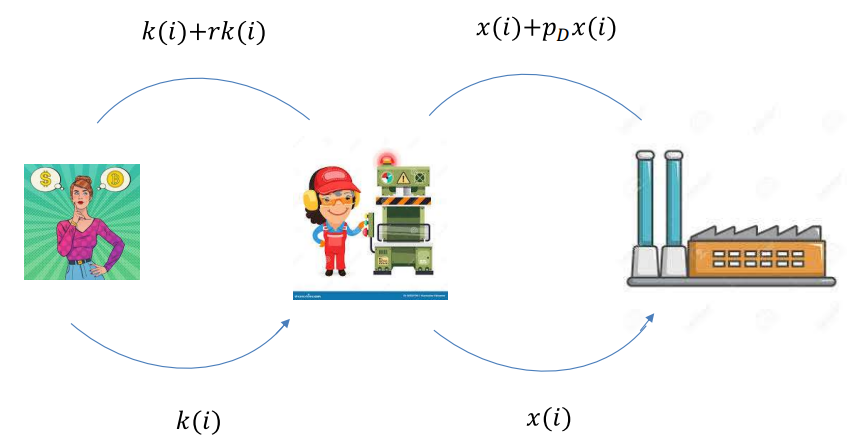
\includegraphics[width=0.7\textwidth]{flows.png}
\end{figure}

\begin{itemize}
    \item The $x$-producer rents differentiated machines to the $Y$-producers. At the end of the period, the $Y$-producer returns these machines plus the rental payment.
    \item The $x$-producer then returns raw capital (transforming $x$'s back into $k$) plus the rental payment to the household. The difference between revenues and costs is the firm's \textbf{profit}.
\end{itemize}

\begin{tcolorbox}[
    colback=blue!1!white,
    colframe=blue!40!white,
    title=The Role of $A$: Returns to Specialization,
    fonttitle=\bfseries
    ]
Consider the discrete version of the production function with intermediate goods index $i \in \{1, \dots, A\}$:
\[
    Y = L^{1-\alpha} \sum_{i=1}^{A} x_i^\alpha, \qquad 0 < \alpha < 1,
\]
subject to the resource constraint
\[
    \sum_{i=1}^{A} x_i = K,
\]
i.e., the total amount of raw capital available is fixed at $K$. Now compare three economies that all share the \textbf{same total input} $K$ but differ in the number of intermediate-goods varieties $A$:
\begin{align*}
    A=1: \quad & Y = L^{1-\alpha} K^\alpha \\[2pt]
    A=2: \quad & Y = L^{1-\alpha} \left[ \left(\tfrac{1}{2} K\right)^\alpha + \left(\tfrac{1}{2} K\right)^\alpha \right] = L^{1-\alpha} \, 2^{1-\alpha} K^\alpha \\[2pt]
    A=3: \quad & Y = L^{1-\alpha} \left[ \left(\tfrac{1}{3} K\right)^\alpha + \left(\tfrac{1}{3} K\right)^\alpha + \left(\tfrac{1}{3} K\right)^\alpha \right] = L^{1-\alpha} \, 3^{1-\alpha} K^\alpha
\end{align*}
The total amount of intermediate goods $A x_i = K$ is \textbf{always the same}; what changes is only how this fixed input is \textit{spread across varieties}. Yet output $Y$ is strictly higher the larger is $A$. The reason is the concavity of $x_i^\alpha$ (with $\alpha < 1$): splitting a fixed input across more varieties avoids diminishing returns within each variety. With $A=1$, diminishing returns set in immediately; with $A=3$, the same total $K$ is distributed over three varieties, each operating in a less-saturated region of its production curve.
\end{tcolorbox}


\subsubsection{R\&D Sector}

Firms in the R\&D sector search for \textbf{ideas} i.e. blueprints / designs, needed by firms for market entry. The market for blueprints is \textbf{perfectly competitive}. Note that the model captures \textit{variety expansion}, not quality expansion.
\\

\noindent The R\&D technology is given by
\[
    \dot{A} = \underbrace{\eta}_{\substack{\text{const. productivity}\\\text{parameter}}} \cdot \underbrace{A}_{\substack{\text{measure of knowledge}\\\text{(intertemp. knowledge spill-over)}}} \cdot \underbrace{L_A}_{\substack{\text{labor in R\&D}\\\text{(private input)}}}
\]
where $\dot{A}$ denotes the number of \textit{newly invented} machine types per unit of time.

\begin{itemize}
    \item $A$ carries \textbf{two meanings} simultaneously: (1) the number of machine \textit{types} which is a technological variable and (2) a \textit{measure of knowledge}. The latter generates the \textbf{intertemporal knowledge spill-over}, i.e. existing knowledge $A$ raises the productivity of researchers $L_A$, so $\dot{A}$ is \textbf{self-amplifying} (premise iii).
    \item \textbf{Why $\dot{A}$ on the LHS and not $A$ (as with $Y$)?} $\rightarrow$ Because $A$ is a \textbf{stock variable} (the number of machine types existing at a point in time), whereas $Y$ is a \textbf{flow variable}. The R\&D technology describes the rate at which new types are added, hence $\dot{A}$.
\end{itemize}

\paragraph{Double knife-edge restriction.} The partial elasticities of $A$ and $L_A$ in the production of $\dot{A}$ are both equal to unity:
\[
    \text{(i)} \quad \frac{\partial \ln \dot{A}}{\partial \ln A} = 1 \qquad \text{and} \qquad \text{(ii)} \quad \frac{\partial \ln \dot{A}}{\partial \ln L_A} = 1.
\]


\subsubsection{General Equilibrium and Reduced Dynamic System}

\subsubsection*{Definition: General Equilibrium}

A general (market) equilibrium for this economy consists of time paths for \textcolor{blue}{\textbf{quantities}}
\[
    \{L_Y(t),\, L_A(t),\, \{x(i,t)\}_{i=0}^{A},\, A(t),\, K(t),\, Y(t),\, a(t),\, C(t)\}_{t=0}^{\infty}
\]
and \textcolor{red}{\textbf{prices}}
\[
    \{w_Y(t),\, w_{RD}(t),\, r(t),\, p_A(t),\, \{p(i,t)\}_{i=0}^{A}\}_{t=0}^{\infty}
\]
such that:
\begin{enumerate}
    \item Final goods producers, intermediate goods producers, and R\&D firms maximize profits $\forall\, t \in [0,\infty]$.
    \item Households maximize lifetime utility $U = \int_0^\infty u(c) \cdot e^{-\rho t}\, dt$.
    \item The capital market \textbf{no-arbitrage condition} holds:
    \[
        \frac{\dot{p}_A}{p_A} + \frac{\pi}{p_A} = r \quad \forall\, t \in [0,\infty].
    \]
    The household holds two assets (equity and raw capital) and must earn the same return on both. The return on equity is the sum of the \textbf{capital gain} $\dot{p}_A/p_A$ and the \textbf{dividend yield} $\pi/p_A$, which must equal the rental rate $r$ on raw capital. Otherwise the household would shift its entire portfolio into the higher-yielding asset.
    \item Capital markets clear: $K(t) = \int_0^A k(i)\, di$, and issued shares $p_A(t) A(t)$ are held by the household $\forall\, t \in [0,\infty]$.
    \item Labor market clears: $L(t) = L_Y(t) + L_A(t) \quad \forall\, t \in [0,\infty]$.
    \item Goods markets clear: $x_S(i) = x_D(i) \;\forall\, i \in [0,A]$ and $Y(t) = I(t) + C(t) \quad \forall\, t \in [0,\infty]$.
\end{enumerate}

\subsubsection*{Reduced Dynamic System}

The equilibrium conditions can be condensed into a system of \textbf{6 equations in 6 endogenous variables}:
\begin{align*}
    \dot{C}     &= \frac{C}{\sigma}(r-\rho)         &&\text{(Keynes-Ramsey rule)} \\
    \dot{p}_A   &= r \cdot p_A - \pi                &&\text{(no-arbitrage condition)} \\
    \dot{A}     &= \eta A L_A                       &&\text{(R\&D technology)} \\
    \dot{a}     &= r \cdot a + w \cdot L - C        &&\text{(wealth accumulation)} \\
    a           &= p_A \cdot A + K                  &&\text{(wealth composition)} \\
    \underbrace{(1-\alpha)(L-L_A)^{-\alpha} A \left(\tfrac{K}{A}\right)^\alpha}_{w_Y} 
                &= \underbrace{p_A \eta A}_{w_{RD}} &&\text{(labor-market arbitrage)}
\end{align*}

\paragraph{Endogenous variables.}
\begin{center}
\begin{tabular}{lll}
    \toprule
    \textbf{Variable} & \textbf{Meaning} & \textbf{Type} \\
    \midrule
    $C$    & consumption                & jump variable \\
    $p_A$  & price of a blueprint       & jump variable \\
    $A$    & ``number'' of blueprints   & state variable \\
    $a$    & wealth                     & jump variable \\
    $K$    & overall capital            & state variable \\
    $L_A$  & labor in R\&D sector       & allocation variable (jump) \\
    \bottomrule
\end{tabular}
\end{center}

\paragraph{Equilibrium relations}
\[
    r = \alpha^2 \frac{Y}{K}; \qquad
    w = (1-\alpha)\frac{Y}{L-L_A}; \qquad
    \pi = (1-\alpha)\alpha \frac{Y}{A}; \qquad
    Y = A^{1-\alpha}(L-L_A)^{1-\alpha} K^\alpha.
\]


\subsubsection{Long-run growth rate}
Along a \textbf{balanced growth path}, the Romer model is equivalent to a neoclassical growth model with labor-augmenting technical progress. Recall the reduced form
\[
    Y = (A L_Y)^{1-\alpha} K^\alpha.
\]
Setting up the reduced dynamic system shows that this is equivalent to a Ramsey model (Use $\dot{K}$, $\dot{C}$, and $\dot{A}$ equations).

\noindent On the balanced growth path, all variables grow at the same rate $g$:
\[
    \hat{Y}^* = \hat{K}^* = \hat{C}^* = \hat{A}^* = g, \qquad \text{where } \hat{X} := \frac{\dot{X}}{X} \text{ for all } X \in \{Y, K, C, A\}.
\]
The long-run growth rate of $A$ (recall $\dot{A} = \eta A L_A$) reads
\[
    \hat{A}^* = \eta L_A^*.
\]
The interesting question therefore concerns the \textbf{determination of $L_A^*$}, since it pins down the long-run growth rate.

\subsubsection{Solution strategy for the balanced growth path}

The steady-state growth rate is determined by combining a production-side and a consumption-side relation:
\begin{enumerate}
    \item The labor-market equilibrium condition $w_Y = w_{RD}$ yields a relation $r_{\text{prod}} = f(g)$ describing \textbf{equilibrium on the production side}.
    \item The Keynes-Ramsey rule yields $r_{\text{cons}} = \sigma g + \rho$, describing \textbf{equilibrium on the consumption side}.
    \item \textbf{Simultaneous equilibrium} on both sides ($r_{\text{prod}} = r_{\text{cons}}$) then allows determination of $r$ and $g$.
\end{enumerate}



\subsubsection{Equilibrium in the labor market $w_Y = w_{RD}$}
Under perfect competition, labor earns its \textbf{value marginal product} (note that the final-good price is the numéraire $p_Y = 1$):
\[
    w_Y = p_Y \frac{\partial Y}{\partial L_Y} = (1-\alpha) L_Y^{-\alpha} A x^\alpha,
\]
recalling that in symmetric equilibrium the technology reads $Y = L_Y^{1-\alpha} A x^\alpha$. For the R\&D sector, the wage equals the value of the marginal contribution to invention:
\[
    w_{RD} = p_A \frac{\partial \dot{A}}{\partial L_A} = p_A \eta A.
\]
The remaining task is to determine the \textbf{price of blueprints} $p_A$.

\subsubsection{Price of a blueprint and equilibrium profits}

Since $\pi$ and $r$ are constant in the steady state, the blueprint price equals the present value of the firm's profit stream:
\[
    p_A(t) = \int_t^\infty \underbrace{\pi(\tau)}_{\text{profit at }\tau \geq t} \cdot \underbrace{e^{-\int_t^\tau r(u)\,du}}_{\text{cumulative discount factor}} d\tau.
\]
With both $\pi$ and $r$ constant, this simplifies to
\[
    p_A(t) = \int_t^\infty \pi e^{-r(\tau - t)}\,d\tau = \frac{\pi}{r}.
\]

\begin{tcolorbox}[
    colback=red!1!white,
    colframe=red!40!white,
    title=Key Result: Price of a Blueprint,
    fonttitle=\bfseries
    ]
In the steady state, the blueprint price equals the discounted profit stream of the intermediate-goods firm:
\[
    \boxed{\, p_A = \frac{\pi}{r} \,}
\]
This pins down the value of the firm and is the \textbf{link between the R\&D sector and the rest of the model}.
\end{tcolorbox}

\paragraph{Profit of the $x$-producer.} The intermediate-goods firm earns
\[
    \pi = \underbrace{p_D(x)}_{\substack{\text{rental price paid}\\\text{by }Y\text{-producer}}} x - r x, \qquad \text{with } p_D(x) = \alpha L_Y^{1-\alpha} x^{\alpha-1}. \qquad (**)
\]
Since the $x$-producer is a monopolist in its variety, it chooses the supply price as a markup $1/\alpha$ over marginal cost $r$:
\[
    p_S = \frac{1}{\alpha} r.
\]
In equilibrium $p_D = p_S$, hence $r = \alpha p_S$, which combined with $(**)$ gives equilibrium profits
\[
    \pi = (p_D - \alpha p_S) x = (1-\alpha) p_D x = (1-\alpha)\alpha L_Y^{1-\alpha} x^\alpha.
\]

\begin{tcolorbox}[
    colback=blue!1!white,
    colframe=blue!40!white,
    title=Derivation: Demand Curve $p_D(x) = \alpha L_Y^{1-\alpha} x^{\alpha-1}$,
    fonttitle=\bfseries
    ]
The demand curve for intermediate good $i$ follows from the final-good producer's profit-maximization problem.

\textit{Discrete case.} The $Y$-producer solves
\[
    \max_{x_i} \; L^{1-\alpha} \sum_{i=1}^A x_i^\alpha - \sum_{i=1}^A p_i x_i.
\]
The first-order condition with respect to $x_i$ gives
\[
    \alpha L^{1-\alpha} x_i^{\alpha-1} = p_i \quad \Longrightarrow \quad p_D(x_i) = \alpha L^{1-\alpha} x_i^{\alpha-1}.
\]

\textit{Continuous case.} The problem becomes
\[
    \max_{x(\cdot)} \int_0^A \left[ L_Y^{1-\alpha} x(i)^\alpha - p(i) x(i) \right] di.
\]
Differentiating under the integral sign yields the same inverse demand function
\[
    p(i) = \alpha L_Y^{1-\alpha} x(i)^{-\alpha+1\cdot(-1)} = \alpha L_Y^{1-\alpha} x(i)^{\alpha-1}.
\]
The $x$-producer takes this demand curve as given when choosing its profit-maximizing supply price.
\end{tcolorbox}

\begin{tcolorbox}[
    colback=blue!1!white,
    colframe=blue!40!white,
    title=Derivation: Monopoly Markup $p_S = r/\alpha$,
    fonttitle=\bfseries
    ]
The $x$-producer is a monopolist in its variety and faces the inverse demand curve $p_D(x) = \alpha L_Y^{1-\alpha} x^{\alpha-1}$ derived from the $Y$-producer's optimization. Its profit-maximization problem is
\[
    \max_x \; \pi = p_D(x)\, x - r x = \alpha L_Y^{1-\alpha} x^\alpha - r x,
\]
where the marginal cost of producing one unit of $x$ equals the rental rate $r$ (recall the linear technology $x(i) = k(i)$).

The first-order condition with respect to $x$ is
\[
    \alpha^2 L_Y^{1-\alpha} x^{\alpha-1} - r = 0 \quad \Longrightarrow \quad \alpha \cdot \underbrace{\alpha L_Y^{1-\alpha} x^{\alpha-1}}_{= p_S} = r.
\]
Solving for the optimal supply price:
\[
    \boxed{\; p_S = \frac{1}{\alpha} r \;}
\]
The monopolist charges a \textbf{markup} of $1/\alpha > 1$ over marginal cost $r$. The markup is larger the smaller is $\alpha$, i.e., the less substitutable the varieties are -- standard monopoly intuition.
\end{tcolorbox}


\subsubsection{Equilibrium on the production side}

Plugging $p_A = \pi/r$ and the equilibrium profit into $w_{RD} = p_A \eta A$, and equating with $w_Y$:
\[
    \underbrace{(1-\alpha) L_Y^{-\alpha} A x^\alpha}_{\partial Y/\partial L_Y} \;=\; \underbrace{\frac{(1-\alpha)\alpha L_Y^{1-\alpha} x^\alpha}{r}}_{p_A} \cdot \underbrace{\eta A}_{\partial \dot{A}/\partial L_A}.
\]
Solving for $r$:
\[
    r = \eta \alpha L_Y.
\]
Using labor-market clearing $L_Y = L - L_A$ and the R\&D technology in steady state $L_A = g/\eta$:
\[
    r = \eta \alpha L_Y = \eta \alpha (L - L_A) = \eta \alpha L - \alpha g.
\]
This relation describes \textbf{equilibrium on the production side}. Note that $g$ and $r$ are \textbf{negatively related}: faster growth requires more researchers $L_A$, which leaves fewer workers for the final-goods sector, lowering the marginal product of capital and hence $r$.

\subsubsection{Steady-state growth rate}

Solving the production-side relation $r = \eta\alpha L - \alpha g$ together with the consumption-side Keynes-Ramsey relation $r = \sigma g + \rho$ for $g$:
\[
    \eta\alpha L - \alpha g = \sigma g + \rho \quad \Longrightarrow \quad g = \frac{\eta\alpha L - \rho}{\sigma + \alpha}.
\]
Since growth cannot turn negative in this model, the complete solution is

\begin{tcolorbox}[
    colback=red!1!white,
    colframe=red!40!white,
    title=Key Result: Romer Steady-State Growth Rate,
    fonttitle=\bfseries
    ]
\[
    \boxed{\; g_M = \begin{cases} \dfrac{\eta\alpha L - \rho}{\sigma + \alpha} & \text{for } \eta\alpha L > \rho \\[4pt] 0 & \text{for } \eta\alpha L \leq \rho \end{cases} \;}
\]
\textbf{Threshold condition.} Long-run growth requires the economy to be \textit{large enough} in the sense $\eta \alpha L > \rho$ (critical threshold for labor).

\textbf{Scale effect.} Provided $\eta \alpha L > \rho$, larger economies (size measured by $L$) grow at a higher rate. Intuition: more researchers can be employed without sacrificing too much final-good production, so $\dot{A}$ is higher.
\end{tcolorbox}

\begin{tcolorbox}[
    colback=darkgreen!1!white,
    colframe=darkgreen!40!white,
    title=Nice to Know: Romer's H vs. L,
    fonttitle=\bfseries
    ]
In the original Romer (1990) paper, there is \textbf{human capital} ($H$) and \textbf{unskilled labor} ($L$), so that both the threshold effect and the scale effect are associated with \textit{human capital} rather than (unskilled) labor. 
\end{tcolorbox}


\subsubsection{Graphical illustration: labor market equilibrium.} Varying only $L_Y$ (holding $x$, $A$, $r$ constant), the wage in the $Y$-sector $w_Y = (1-\alpha) L_Y^{-\alpha} A x^\alpha$ is decreasing in $L_Y$, while the R\&D wage $w_{RD} = \frac{(1-\alpha)\alpha L_Y^{1-\alpha} x^\alpha}{r} \eta A$ is increasing in $L_Y$. Their intersection determines the equilibrium allocation between $L_Y$ and $L_A$ (recall $L_A = L - L_Y$).
\begin{figure}[H]
    \centering
    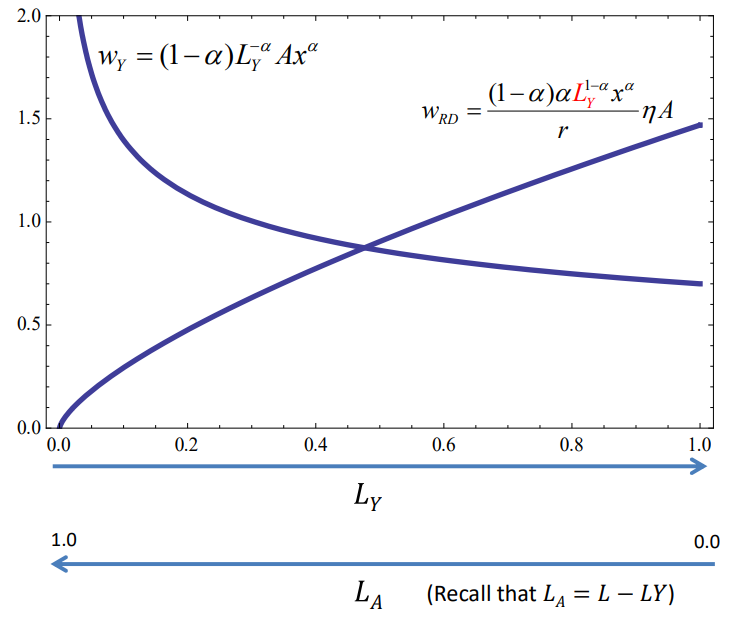
\includegraphics[width=0.55\textwidth]{labor_market_eq_I.png}
\end{figure}

\paragraph{Why does $w_{RD}$ increase in $L_Y$?} A higher $L_Y$ raises the marginal product of intermediate goods $x$, which raises profits $\pi$ of the $x$-producer, which raises the value $p_A = \pi/r$ of a blueprint, which in turn raises the value marginal product of labor in R\&D ($w_{RD} = p_A \eta A$).

\paragraph{Wage subsidy.} If the government subsidizes R\&D wages at rate $s_A$, the FOC of the typical R\&D firm becomes
\[
    (1-s_A) w_{RD} = \frac{(1-\alpha)\alpha L_Y^{1-\alpha} x^\alpha}{r} \eta A \quad \Longrightarrow \quad w_{RD} = \frac{(1-\alpha)\alpha L_Y^{1-\alpha} x^\alpha}{r(1-s_A)}\eta A.
\]
The $w_{RD}$-curve shifts up, the equilibrium moves toward higher $L_A$ and lower $L_Y$, raising the steady-state growth rate.
\begin{figure}[H]
    \centering
    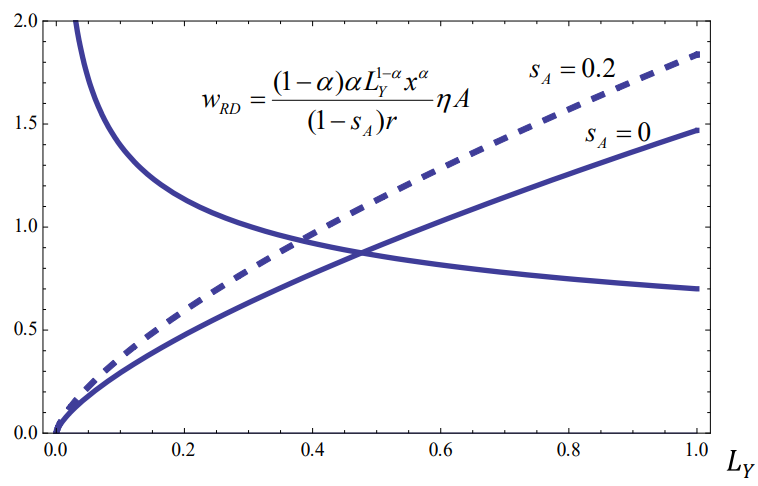
\includegraphics[width=0.55\textwidth]{labor_market_eq_II.png}
\end{figure}

\begin{tcolorbox}[
    colback=blue!1!white,
    colframe=blue!40!white,
    title=Derivation: Effect of an R\&D Wage Subsidy,
    fonttitle=\bfseries
    ]
Suppose the government subsidizes R\&D wages at rate $s_A$. The subsidy is paid to the \textbf{R\&D firm}: workers still receive the market wage $w_{RD}$, but the firm only pays $(1-s_A) w_{RD}$ per researcher, with the government covering the remainder $s_A w_{RD}$.
\\\\
R\&D firm's problem, taking $w_{RD}$ as given:  
\[
    \max_{L_A} \; \Big\{\, p_A \dot{A}(L_A) \;-\; (1-s_A)\, w_{RD}\, L_A \,\Big\}, \qquad \text{with } \dot{A}(L_A) = \eta A L_A.
\]
The first-order condition with respect to $L_A$ is
\[
    p_A \cdot \frac{\partial \dot{A}}{\partial L_A} = (1-s_A) w_{RD} \quad \Longrightarrow \quad p_A \eta A = (1-s_A) w_{RD}.
\]
Solving for $w_{RD}$ and substituting $p_A = \pi/r = (1-\alpha)\alpha L_Y^{1-\alpha} x^\alpha / r$:
\[
    w_{RD} = \frac{p_A \eta A}{1-s_A} = \frac{(1-\alpha)\alpha L_Y^{1-\alpha} x^\alpha}{r(1-s_A)}\, \eta A.
\]

The subsidy corrects the two market imperfections (knowledge spill-over + incomplete appropriation of consumer surplus) that cause the decentralized growth rate $g_M$ to fall short of the socially optimal $g_S$. The subsidy pushes $g_M$ towards $g_S$.
\end{tcolorbox}

\paragraph{Graphical determination of $g$ and $r$.} The simultaneous equilibrium can be plotted in $(r,g)$-space. The production-side relation $g = (\eta\alpha L - r)/\alpha$ is downward-sloping; the consumption-side relation $g = (r-\rho)/\sigma$ is upward-sloping. Their intersection determines $(r^*, g^*)$.

\begin{figure}[H]
    \centering
    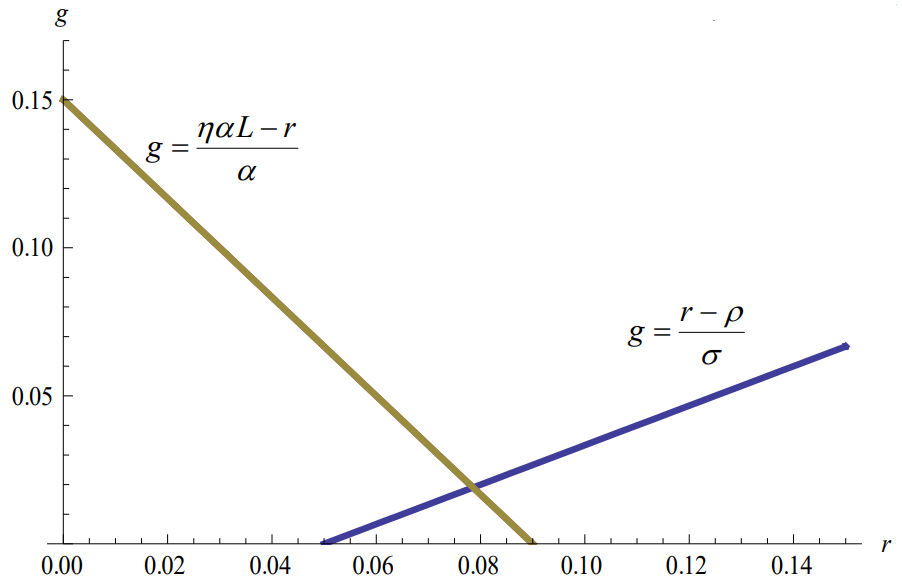
\includegraphics[width=0.55\textwidth]{g_r_diagram.png}
\end{figure}
\begin{tcolorbox}[
    colback=blue!1!white,
    colframe=blue!40!white,
    title=Exercise: Effect of $s_A = 0.2$ on the $g$-$r$ Diagram,
    fonttitle=\bfseries
    ]
With a wage subsidy, the production-side relation becomes
\[
    g = \frac{\eta\alpha L - r(1-s_A)}{\alpha},
\]
while the consumption-side relation $g = (r-\rho)/\sigma$ is unaffected.
\\\\
Graphical effect: The production-side curve rotates: its slope flattens from $-1/\alpha$ to $-(1-s_A)/\alpha$, and its $r$-intercept shifts outward from $\eta\alpha L$ to $\eta\alpha L/(1-s_A)$. The consumption-side curve stays fixed.
\\\\
Solving simultaneously yields
\[
    g^* = \frac{\eta\alpha L - \rho(1-s_A)}{\sigma(1-s_A) + \alpha}, \qquad r^* = \frac{\sigma\eta\alpha L + \alpha\rho}{\sigma(1-s_A) + \alpha}.
\]
Both $g^*$ and $r^*$ \textbf{rise} relative to the no-subsidy benchmark. The subsidy lowers the effective labor cost of R\&D firms, who hire more researchers. Hence $L_A$ rises, $\dot{A} = \eta A L_A$ rises, and so does steady-state growth $g$. The interest rate rises along the Keynes-Ramsey rule and faster consumption growth requires a higher return on saving to keep households on their optimal path. Equivalently, on the production side, less labor in the $Y$-sector raises the marginal product of capital and thus $r$.
\end{tcolorbox}
\subsubsection{Market imperfections and policy implications}

The decentralized solution $g_M$ is generically inefficient. Solving the social planner's problem (this is an exercise) yields

\begin{tcolorbox}[
    colback=red!1!white,
    colframe=red!40!white,
    title=Key Result: Social Planner's Solution,
    fonttitle=\bfseries
    ]
\[
    g_S = \begin{cases} \dfrac{\eta L - \rho}{\sigma} & \text{for } \eta L > \rho \\[4pt] 0 & \text{for } \eta L \leq \rho \end{cases}
\]
The decentralized growth rate is \textbf{too low}: $g_M < g_S$.
\end{tcolorbox}

\paragraph{Two market imperfections related to R\&D.}
\begin{itemize}
    \item \textbf{Intertemporal knowledge spill-over effect.} Each new blueprint raises future research productivity (recall the R\&D technology $\dot{A} = \eta A L_A$). This social benefit is \textbf{not reflected in the market price} $p_A = \pi/r$: the inventor only captures the private profit stream, not the contribution to future researchers' productivity.
    \item \textbf{Incomplete appropriation of consumer surplus.} The typical intermediate-goods producer realizes \textbf{monopoly profits} -- this imperfection is in fact \textit{necessary} for market-based R\&D, since otherwise the blueprint would have zero value. However, the monopolist \textbf{cannot appropriate the entire consumer surplus}. Hence, again, the market price $p_A = \pi/r$ falls short of the social value of the blueprint.
\end{itemize}

\noindent Both imperfections imply that R\&D investment is \textbf{suboptimally low} in the decentralized equilibrium. The deviation of the decentralized solution from the first-best calls for \textbf{government intervention}, e.g., R\&D subsidies (such as the wage subsidy $s_A$ analyzed above) that align $g_M$ with $g_S$.